\toclesssection{Hashing}

\toclesssubsection{Recapitulation}

\begin{frame}{Hashing}{Recapitulation}
  \onslide<1->
  \textbf{Hashing:}
  \begin{itemize}   
  \item<2->
    No hash function is good for all key sets!\\
    \begin{itemize}
    \item<3->
      This cannot work, because a big universe
      is mapped onto a small set: {\color{MainA}$\vert \mathbb{U} \vert > m$}
    \end{itemize}
  \item<4->
    For random key sets also simple hash function work, e.g.
     {\color{MainA}\[\Rightarrow h(x) = x \mod m\]}\vspace*{-2em}
     \begin{itemize}
    \item<5->
      Then the random keys make sure that it is distributed evenly
     \end{itemize}
  \item<6->
   To find a good hash function for every key set universal hashing is needed
     \begin{itemize}
    \item<7->
      Then however, for a fixed set of keys not every hash function is suitable,
      but only some
    \end{itemize}
  \end{itemize}
\end{frame}

%-------------------------------------------------------------------------------

\begin{frame}{Hashing}{Recapitulation}
  \textbf{Rehashing:}
  \begin{itemize}
    \item<2->
      It is possible to get bad hash functions with universal hashing, but it
      is unlikely
    \item<3->
      This is determinable by monitoring the maximum bucket size

    \item<4-> If a pre-defined level is exceeded, then a {\color{MainA}rehash} is performed
  \end{itemize}
  \onslide<5->
  \textbf{How to rehash?}
  \begin{itemize}
    \item<5->
      New hash table with a new random hash function
    \item<6->
      Copy elements into the new table
      \begin{itemize}
        \item<7->
          Expensive but happens not often
        \item<8->
          Therefore the average cost is low
        \item<9->
          Look at {\color{MainA}amortized analysis} in the next lecture
      \end{itemize}
  \end{itemize}
\end{frame}

%-------------------------------------------------------------------------------

\subsection{Treatment of hash collisions}

\begin{frame}{Hashing}{Linked List}
  \textbf{Buckets as linked list:}
  \begin{itemize}
    \item<2->
      Each bucket is a linked list
    \item<3->
      Colliding keys are inserted into the linked list of a bucket, either sorted or appended at the end
  \onslide<4->
%  \vspace*{-1.0em}
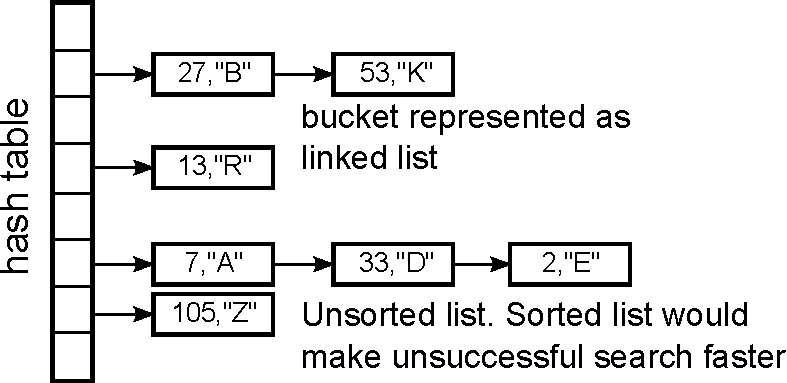
\includegraphics[height=0.35\textheight]{Images/hashtable-buckets.pdf}
  % \begin{table}[!b]
  %   \label{tab:hashing:linked_list:hash_table}
  %   \begin{tabularx}{0.875\textwidth}{c|l}
  %     Bucket & Value\\
  %     \midrule
  %     0 & \lstinline[
  %       language=Python,
  %       style={python-idle-code},
  %       basicstyle=\small
  %     ]|None|\\
  %     1 &
  %     \lstinline[
  %       language=Python,
  %       style={python-idle-code},
  %       mathescape=true,
  %       basicstyle=\small
  %     ]|(3126, "B") $\rightarrow$ (4561, "D") $\rightarrow$ None|\\
  %     2 &
  %     \lstinline[
  %       language=Python,
  %       style={python-idle-code},
  %       mathescape=true,
  %       basicstyle=\small
  %     ]|(5147, "C") $\rightarrow$ None|\\
  %     3 &
  %     \lstinline[
  %       language=Python,
  %       style={python-idle-code},
  %       mathescape=true,
  %       basicstyle=\small
  %     ]|(3903, "A") $\rightarrow$ (1683, "D")
  %       $\rightarrow$ (4818, "E")
  %       $\rightarrow$ None|\\
  %     4 & \lstinline[
  %       language=Python,
  %       style={python-idle-code},
  %       basicstyle=\small
  %     ]|None|\\
  %   \end{tabularx}
  % \end{table}
   \item<5->
     Operations in {\color{MainA}$O(1)$} are possible if a suitable tablesize and hashfunction is
     selected
   \item<6->
     Worst case {\color{MainA}$O(n)$}, e.g. tablesize of 1
   \item<7->
     Dynamic number of elements is possible 
  \end{itemize}
\end{frame}

%-------------------------------------------------------------------------------

\subsection{Open Addressing}

\begin{frame}{Hashing}{Open Addressing}
  \begin{itemize}
    \item<1->
      For colliding keys we choose a new free entry
    \item<2->
      Static, fixed number of elements
    \item<3->
      The \textbf{probe sequence} determines for each key, in which sequence
      all hash table entries are searched for a free bucket
      \begin{itemize}
      \item<4->
        If a entry is already occupied, then iteratively the
        {\color{MainA}following entry} can be checked.
        If a free entry is found the element is inserted
      \item<5->
        If element is not found at the corresponding table entry, even if
        the entry is occupied, then probing has to be performed until
        the element or a free entry have been found
    \end{itemize}
  \end{itemize}
\end{frame}

%-------------------------------------------------------------------------------

\begin{frame}{Hashing}{Open Addressing}
  \textbf{Definitions:}
  \begin{itemize}
    \item<2->[\color{MainA}$h(s)$]
      Hash function for key {\color{MainA}$s$}
    \item<3->[\color{MainA}$g(s,j)$]
      Probing function for key {\color{MainA}$s$}
      with overflow positions {\color{MainA}$j \in \{0,\dots,m-1\}$}
      e.g. {\color{MainA}g(s,j)=j}
    \item<4->
      The \textbf{probe sequence } is calculated by
      \begin{displaymath}
        {\color{MainA}h(s,j)}
        = ({\color{MainA}h(s)} - {\color{MainA}g(s,j)})
        \mod m \in \{0,\dots,m-1\}
      \end{displaymath}
  \end{itemize}
  \vspace{-1em}
  \begin{center}
    \begin{adjustbox}{width=0.75\linewidth}%
      \onslide<4->\begin{tikzpicture}[
  bucket/.style={
    draw={Mittel-Blau},
    fill={white},
    line width=0.075em
  }, bucket_text/.style={
    draw=none,
    color=black
  }, arrow_taken/.style={
    draw={Mittel-Gruen},
    line width=0.125em
  }, arrow_shadow/.style={
    draw={Mittel-Gruen!40!white},
    line width=0.125em
  }, hash_text/.style={
    draw=none,
    color={Mittel-Blau}
  }, hash_text_final/.style={
    draw=none,
    color={Mittel-Blau}
  }
]%

\foreach \x/\xi in
    {\relax/0,${\color{Mittel-Blau}s}$/1,X/2,X/3,X/4,X/5,\relax/6}{
  \draw[bucket]
    (\xi, 0.0) rectangle (\xi + 1.0, 0.5);
  \draw (\xi + 0.5, 0.25) node[bucket_text] {\x};
  \draw (\xi + 0.5, 0.5) node[bucket_text, anchor=south] {\xi};
}

\foreach \type [count=\xi] in
    {taken}{
  \draw (\xi + 0.45 +4, 1.0) edge[arrow_\type, in=0, out=90] (\xi+4, 1.4);
  \draw (\xi+4, 1.4) edge[->, arrow_\type, in=90, out=180] (\xi +4- 0.45, 1.0);
}


% \draw (0.45, 1.0) edge[arrow_shadow, in=0, out=90] (0, 1.4);
% \draw (7.0, 1.4) edge[->, arrow_shadow, in=90, out=180] (6.55, 1.0);

%\draw (1.5, -0.75) node[hash_text] {$h(s, 4)$};
\draw (5.5, -0.75) node[hash_text_final] {$h(s)$};
\draw (5.5, -0.5) edge[->, arrow_taken, color={Mittel-Blau}] (5.5, -0.1);
\end{tikzpicture}%%
    \end{adjustbox}
  \end{center}
\end{frame}

%-------------------------------------------------------------------------------

\codeslide{python}{
\begin{frame}{Hashing}{Open Addressing - Python}
  \lstinputlisting[
    language=Python,
    basicstyle=\small,
    tabsize=4,
    style={python-idle-code},
    breaklines=false,
    emph={insert, None, h, g},
    emphstyle=\color{blue}
  ]{Code/OpenHashing_Insert.py}
\end{frame}

%-------------------------------------------------------------------------------

\begin{frame}{Hashing}{Open Addressing - Python}
  \lstinputlisting[
    language=Python,
    basicstyle=\small,
    tabsize=4,
    style={python-idle-code},
    breaklines=false,
    emph={lookup, None, h, g},
    emphstyle=\color{blue}
  ]{Code/OpenHashing_Lookup.py}
\end{frame}
}

%-------------------------------------------------------------------------------

\codeslide{java}{
\begin{frame}{Hashing}{Open Addressing - Java}
  \lstinputlisting[
    language=Java,
    basicstyle=\scriptesize,
    tabsize=4,
    style={java-eclipse-code},
    breaklines=false,
    mathescape=true,
    escapechar={@},
    emph={j},
    emphstyle=\color{java_variable}
  ]{Code/OpenHashing_Insert.java}
\end{frame}

%-------------------------------------------------------------------------------

\begin{frame}{Hashing}{Open Addressing - Java}
  \lstinputlisting[
    language=Java,
    basicstyle=\scriptesize,
    tabsize=4,
    style={java-eclipse-code},
    breaklines=false,
    mathescape=true,
    escapechar={@},
    emph={j},
    emphstyle=\color{java_variable}
  ]{Code/OpenHashing_Lookup.java}
\end{frame}
}

%-------------------------------------------------------------------------------

\codeslide{cpp}{
\begin{frame}{Hashing}{Open Addressing - C++}
  \lstinputlisting[
    language=C++,
    basicstyle=\small,
    tabsize=2,
    style={cpp-eclipse-code},
    breaklines=false,
    escapechar={@}
  ]{Code/OpenHashing_Insert.cpp}
\end{frame}

%-------------------------------------------------------------------------------

\begin{frame}{Hashing}{Open Addressing - C++}
  \lstinputlisting[
    language=C++,
    basicstyle=\small,
    tabsize=2,
    style={cpp-eclipse-code},
    breaklines=false,
    morekeywords={nullptr},
    escapechar={@}
  ]{Code/OpenHashing_Lookup.cpp}
\end{frame}
}

%-------------------------------------------------------------------------------

\begin{frame}{Hashing}{Open Addressing - Linear Probing}
  \begin{figure}[!h]
    \begin{adjustbox}{width=0.75\linewidth}%
      \begin{adjustbox}{width=0.75\linewidth}%
\begin{tikzpicture}[
  bucket/.style={
    draw={Mittel-Blau},
    fill={white},
    line width=0.075em
  }, bucket_text/.style={
    draw=none,
    color=black
  }, arrow_taken/.style={
    draw={Mittel-Gruen},
    line width=0.125em
  }, arrow_shadow/.style={
    draw={Mittel-Gruen!40!white},
    line width=0.125em
  }, hash_text/.style={
    draw=none,
    color={Mittel-Blau}
  }, hash_text_final/.style={
    draw=none,
    color={Mittel-Blau}
  }
]%
\foreach \x/\xi in
    {\relax/0,${\color{Mittel-Blau}s}$/1,X/2,X/3,X/4,X/5,\relax/6}{
  \draw[bucket]
    (\xi, 0.0) rectangle (\xi + 1.0, 0.5);
  \draw (\xi + 0.5, 0.25) node[bucket_text] {\x};
  \draw (\xi + 0.5, 0.5) node[bucket_text, anchor=south] {\xi};
}

\foreach \type [count=\xi] in
    {shadow,taken,taken,taken,taken}{
  \draw (\xi + 0.45, 1.0) edge[arrow_\type, in=0, out=90] (\xi, 1.4);
  \draw (\xi, 1.4) edge[->, arrow_\type, in=90, out=180] (\xi - 0.45, 1.0);
}

\draw (0.45, 1.0) edge[arrow_shadow, in=0, out=90] (0, 1.4);
\draw (7.0, 1.4) edge[->, arrow_shadow, in=90, out=180] (6.55, 1.0);

\draw (1.5, -0.75) node[hash_text] {$h(s, 4)$};
\draw (5.5, -0.75) node[hash_text_final] {$h(s, 0)$};
\draw (1.5, -0.5) edge[->, arrow_taken, color={Mittel-Blau}] (1.5, -0.1);
\draw (5.5, -0.5) edge[->, arrow_taken] (5.5, -0.1);
\end{tikzpicture}%
\end{adjustbox}%%
    \end{adjustbox}
    \vspace{-1.0em}
    \caption{Linear probe sequence}%
    \label{fig:hashing:open_addressing:linear_probing}%
  \end{figure}
  \vspace{-1.0em}
  \begin{itemize}
    \item<2->
      Check the element with lower index:
      \begin{math}
        {\color{MainA}g(s,j)} := {\color{MainA}j}
      \end{math}\\
      $\Rightarrow$ Hash function:
      \begin{math}
        {\color{MainA}h(s,j)}
        = ({\color{MainA}h(s)} - {\color{MainA}j}) \mod m
      \end{math}
    \item<3->
      This leads to the following probe sequence
      \begin{displaymath}
        {\color{MainA}h(s)},
        {\color{MainA}h(s)}-1,
        {\color{MainA}h(s)}-2,
        \dots,
        \underbrace{0, m-1}_\text{clipping},
        m-2,
        \dots,
        {\color{MainA}h(s)}+1
      \end{displaymath}
  \end{itemize}
\end{frame}

%-------------------------------------------------------------------------------

\begin{frame}{Hashing}{Open Addressing - Linear Probing}
  \begin{figure}[!h]
    \begin{adjustbox}{width=0.75\linewidth}%
      \begin{adjustbox}{width=0.75\linewidth}%
\begin{tikzpicture}[
  bucket/.style={
    draw={Mittel-Blau},
    fill={white},
    line width=0.075em
  }, bucket_text/.style={
    draw=none,
    color=black
  }, arrow_taken/.style={
    draw={Mittel-Gruen},
    line width=0.125em
  }, arrow_shadow/.style={
    draw={Mittel-Gruen!40!white},
    line width=0.125em
  }, hash_text/.style={
    draw=none,
    color={Mittel-Blau}
  }, hash_text_final/.style={
    draw=none,
    color={Mittel-Blau}
  }
]%
\foreach \x/\xi in
    {\relax/0,${\color{Mittel-Blau}s}$/1,X/2,X/3,X/4,X/5,\relax/6}{
  \draw[bucket]
    (\xi, 0.0) rectangle (\xi + 1.0, 0.5);
  \draw (\xi + 0.5, 0.25) node[bucket_text] {\x};
  \draw (\xi + 0.5, 0.5) node[bucket_text, anchor=south] {\xi};
}

\foreach \type [count=\xi] in
    {shadow,taken,taken,taken,taken}{
  \draw (\xi + 0.45, 1.0) edge[arrow_\type, in=0, out=90] (\xi, 1.4);
  \draw (\xi, 1.4) edge[->, arrow_\type, in=90, out=180] (\xi - 0.45, 1.0);
}

\draw (0.45, 1.0) edge[arrow_shadow, in=0, out=90] (0, 1.4);
\draw (7.0, 1.4) edge[->, arrow_shadow, in=90, out=180] (6.55, 1.0);

\draw (1.5, -0.75) node[hash_text] {$h(s, 4)$};
\draw (5.5, -0.75) node[hash_text_final] {$h(s, 0)$};
\draw (1.5, -0.5) edge[->, arrow_taken, color={Mittel-Blau}] (1.5, -0.1);
\draw (5.5, -0.5) edge[->, arrow_taken] (5.5, -0.1);
\end{tikzpicture}%
\end{adjustbox}%%
    \end{adjustbox}
    \vspace{-0.5em}
    \caption{Linear probe sequence}%
    \label{fig:hashing:open_addressing:linear_probing2}%
  \end{figure}
  \vspace{-1.5em}
  \begin{itemize}
    \item<2->
      Can result in primary clustering
    \item<3->
      Dealing with a hash collision will result in a higher probability of hash
      collisions in close entries
  \end{itemize}
\end{frame}

%-------------------------------------------------------------------------------

\begin{frame}{Hashing}{Open Addressing - Linear Probing}
  \textbf{Example:}
  \begin{itemize}
    \item<2->
      Keys:
        \begin{math}
          {\color{MainA}
         \{12, 53, 5, 15, 2, 19\}}
      \end{math}
    \item<3->
      Hash function:
      \begin{math}
        {\color{MainA}h(s,j)
        = (s \mod 7 - j) \mod 7}
      \end{math}
  \end{itemize}
  \hfill\\[0.5em]
   \begin{itemize}
    \item<4->
      \lstinline[
        language=Python,
        style={python-idle-code},
        mathescape=true,
        basicstyle=\small
      ]|t.insert(12, "A")|$,\;$
      \begin{math}
        {\color{MainA}h(12, 0)} = 5
      \end{math}
      \begin{figure}[!h]
        \def\LPEData{
          \relax/0,
          \relax/1,
          \relax/2,
          \relax/3,
          \relax/4,
          {12, {\color{green2}A}}/5,
          \relax/6
        }%
        \def\LPEShowIndex{1}%
        \begin{adjustbox}{width=0.75\linewidth}%
          \begin{tikzpicture}[
  bucket/.style={
    draw={Mittel-Blau},
    fill={white},
    line width=0.075em
  }, bucket_text/.style={
    draw=none,
    color=black
  }
]%
\foreach \x/\xi in \LPEData {
  \draw[bucket]
    (\xi, 0.0) rectangle (\xi + 1.0, 0.5);
  \draw (\xi + 0.5, 0.25) node[bucket_text] {\x};
  
  \ifnum \LPEShowIndex>0
    \draw (\xi + 0.5, 0.5) node[bucket_text, anchor=south] {\xi};
  \fi
}
\end{tikzpicture}%%
        \end{adjustbox}
        \vspace{-0.5em}%
%        \caption{Probe sequence}%
        \label{fig:hashing:open_addressing:linear_probing_example}%
      \end{figure}
      \hfill\\[1.0em]
    \item<5->
      \lstinline[
        language=Python,
        style={python-idle-code},
        mathescape=true,
        basicstyle=\small
      ]|t.insert(53, "B")|$,\;$
      \begin{math}
        {\color{MainA}h(53, 0)} = 4
      \end{math}
      \begin{figure}[!h]
        \def\LPEData{
          \relax/0,
          \relax/1,
          \relax/2,
          \relax/3,
          {53, {\color{green2}B}}/4,
          {12, {\color{green2}A}}/5,
          \relax/6
        }%
        \def\LPEShowIndex{0}%
        \begin{adjustbox}{width=0.75\linewidth}%
          \begin{tikzpicture}[
  bucket/.style={
    draw={Mittel-Blau},
    fill={white},
    line width=0.075em
  }, bucket_text/.style={
    draw=none,
    color=black
  }
]%
\foreach \x/\xi in \LPEData {
  \draw[bucket]
    (\xi, 0.0) rectangle (\xi + 1.0, 0.5);
  \draw (\xi + 0.5, 0.25) node[bucket_text] {\x};
  
  \ifnum \LPEShowIndex>0
    \draw (\xi + 0.5, 0.5) node[bucket_text, anchor=south] {\xi};
  \fi
}
\end{tikzpicture}%%
        \end{adjustbox}
        \vspace{-0.5em}%
        \caption{Probe/Insertion sequence on a hash map}%
        \label{fig:hashing:open_addressing:linear_probing_example2}%
      \end{figure}
  \end{itemize}
\end{frame}

%-------------------------------------------------------------------------------

\begin{frame}{Hashing}{Open Addressing - Linear Probing}
  \textbf{Example:}
  \begin{itemize}
    \item
      Hash function:
      \begin{math}
        {\color{MainA}h(s,j)}
        = ({\color{MainA}s} \mod 7 - {\color{MainA}j}) \mod 7
      \end{math}
  \end{itemize}
  \hfill\\[0.5em]
  \begin{itemize}
    \item<2->
      \lstinline[
        language=Python,
        style={python-idle-code},
        mathescape=true,
        basicstyle=\small
      ]|t.insert(5, "C")|$,\;$
      \begin{math}
        {\color{MainA}h(5, 0)} = 5 ,\;
        {\color{MainA}h(5, 1)} = 4 ,\;
        {\color{MainA}h(5, 2)} = 3
      \end{math}
      \begin{figure}[!h]
        \def\LPEData{
          \relax/0,
          \relax/1,
          \relax/2,
          {5, {\color{green2}C}}/3,
          {53, {\color{green2}B}}/4,
          {12, {\color{green2}A}}/5,
          \relax/6
        }%
        \def\LPEShowIndex{1}%
        \begin{adjustbox}{width=0.75\linewidth}%
          \begin{tikzpicture}[
  bucket/.style={
    draw={Mittel-Blau},
    fill={white},
    line width=0.075em
  }, bucket_text/.style={
    draw=none,
    color=black
  }
]%
\foreach \x/\xi in \LPEData {
  \draw[bucket]
    (\xi, 0.0) rectangle (\xi + 1.0, 0.5);
  \draw (\xi + 0.5, 0.25) node[bucket_text] {\x};
  
  \ifnum \LPEShowIndex>0
    \draw (\xi + 0.5, 0.5) node[bucket_text, anchor=south] {\xi};
  \fi
}
\end{tikzpicture}%%
        \end{adjustbox}
        \vspace{-0.5em}%
%        \caption{Insertion sequence}%
        \label{fig:hashing:open_addressing:linear_probing_example3}%
      \end{figure}
      \hfill\\[1.0em]
    \item<3->
      \lstinline[
        language=Python,
        style={python-idle-code},
        mathescape=true,
        basicstyle=\small
      ]|t.insert(15, "D")|$,\;$
      \begin{math}
        {\color{MainA}h(15, 0)} = 1
      \end{math}
      \begin{figure}[!h]
        \def\LPEData{
          \relax/0,
          {15, {\color{green2}D}}/1,
          \relax/2,
          {5, {\color{green2}C}}/3,
          {53, {\color{green2}B}}/4,
          {12, {\color{green2}A}}/5,
          \relax/6
        }%
        \def\LPEShowIndex{0}%
        \begin{adjustbox}{width=0.75\linewidth}%
          \begin{tikzpicture}[
  bucket/.style={
    draw={Mittel-Blau},
    fill={white},
    line width=0.075em
  }, bucket_text/.style={
    draw=none,
    color=black
  }
]%
\foreach \x/\xi in \LPEData {
  \draw[bucket]
    (\xi, 0.0) rectangle (\xi + 1.0, 0.5);
  \draw (\xi + 0.5, 0.25) node[bucket_text] {\x};
  
  \ifnum \LPEShowIndex>0
    \draw (\xi + 0.5, 0.5) node[bucket_text, anchor=south] {\xi};
  \fi
}
\end{tikzpicture}%%
        \end{adjustbox}
        \vspace{-0.5em}%
        \caption{Probe/Insertion sequence on a hash map}%
        \label{fig:hashing:open_addressing:linear_probing_example4}%
      \end{figure}
  \end{itemize}
\end{frame}

%-------------------------------------------------------------------------------

\begin{frame}{Hashing}{Open Addressing - Linear Probing}
  \textbf{Example:}
  \begin{itemize}
    \item
      Hash function:
      \begin{math}
        {\color{MainA}h(s,j)}
        = ({\color{MainA}s} \mod 7 - {\color{MainA}j}) \mod 7
      \end{math}
  \end{itemize}
  \hfill\\[0.5em]
  \begin{itemize}
    \item<2->
      \lstinline[
        language=Python,
        style={python-idle-code},
        mathescape=true,
        basicstyle=\small
      ]|t.insert(2, "E")|$,\;$
      \begin{math}
      {\color{MainA}h(2, 0)} = 2
      \end{math}
      \begin{figure}[!h]
        \def\LPEData{
          \relax/0,
          {15, {\color{green2}D}}/1,
          {2, {\color{green2}E}}/2,
          {5, {\color{green2}C}}/3,
          {53, {\color{green2}B}}/4,
          {12, {\color{green2}A}}/5,
          \relax/6
        }%
        \def\LPEShowIndex{1}%
        \begin{adjustbox}{width=0.75\linewidth}%
          \begin{tikzpicture}[
  bucket/.style={
    draw={Mittel-Blau},
    fill={white},
    line width=0.075em
  }, bucket_text/.style={
    draw=none,
    color=black
  }
]%
\foreach \x/\xi in \LPEData {
  \draw[bucket]
    (\xi, 0.0) rectangle (\xi + 1.0, 0.5);
  \draw (\xi + 0.5, 0.25) node[bucket_text] {\x};
  
  \ifnum \LPEShowIndex>0
    \draw (\xi + 0.5, 0.5) node[bucket_text, anchor=south] {\xi};
  \fi
}
\end{tikzpicture}%%
        \end{adjustbox}
        \vspace{-0.5em}%
%        \caption{Insertion sequence on a hash map}%
        \label{fig:hashing:open_addressing:linear_probing_example6}%
      \end{figure}
      \hfill\\[1.0em]
    \item<3->
      \lstinline[
        language=Python,
        style={python-idle-code},
        mathescape=true,
        basicstyle=\small
      ]|t.insert(19, "F")|$,\;$
      \begin{math}
        {\color{MainA}h(19, 0)} = 5 ,\;
        {\color{MainA}h(19, 1)} = 4 ,\;
      \end{math}\\
      \begin{math}
        \hspace{1.5em}
        {\color{MainA}h(19, 2)} = 3 ,\;
        {\color{MainA}h(19, 3)} = 2 ,\;
        {\color{MainA}h(19, 4)} = 1 ,\;
        {\color{MainA}h(19, 5)} = 0
      \end{math}
      \begin{figure}[!h]
        \def\LPEData{
          {19, {\color{green2}F}}/0,
          {15, {\color{green2}D}}/1,
          {2, {\color{green2}E}}/2,
          {5, {\color{green2}C}}/3,
          {53, {\color{green2}B}}/4,
          {12, {\color{green2}A}}/5,
          \relax/6
        }%
        \def\LPEShowIndex{0}%
        \begin{adjustbox}{width=0.75\linewidth}%
          \begin{tikzpicture}[
  bucket/.style={
    draw={Mittel-Blau},
    fill={white},
    line width=0.075em
  }, bucket_text/.style={
    draw=none,
    color=black
  }
]%
\foreach \x/\xi in \LPEData {
  \draw[bucket]
    (\xi, 0.0) rectangle (\xi + 1.0, 0.5);
  \draw (\xi + 0.5, 0.25) node[bucket_text] {\x};
  
  \ifnum \LPEShowIndex>0
    \draw (\xi + 0.5, 0.5) node[bucket_text, anchor=south] {\xi};
  \fi
}
\end{tikzpicture}%%
        \end{adjustbox}
        \vspace{-0.5em}%
        \caption{Probe/Insertion sequence on a hash map}%
        \label{fig:hashing:open_addressing:linear_probing_example7}%
      \end{figure}
  \end{itemize}
\end{frame}

%-------------------------------------------------------------------------------

\begin{frame}{Hashing}{Open Addressing - Squared Probing}
  \textbf{Squared probing:}
  \begin{itemize}
    \item<2->
      Motivation: Avoid local clustering
      \begin{displaymath}
        {\color{MainA}g(s,j)}
        := (-1)^{\color{MainA}j}
        \left\lceil \frac{{\color{MainA}j}}{2} \right\rceil^2
      \end{displaymath}
    \onslide<3->
    \vspace{-2.0em}
  \begin{figure}[!h]
    \begin{adjustbox}{width=0.7\linewidth}%
      \begin{adjustbox}{width=0.7\linewidth}%
\begin{tikzpicture}[
  bucket/.style={
    draw={Mittel-Blau},
    fill={white},
    line width=0.075em
  }, bucket_text/.style={
    draw=none,
    color=black
  }, arrow_taken/.style={
    draw={Mittel-Gruen},
    line width=0.125em
  }, arrow_shadow/.style={
    draw={Mittel-Gruen!40!white},
    line width=0.125em
  }, hash_text/.style={
    draw=none,
    color={Mittel-Blau}
  }, hash_text_final/.style={
    draw=none,
    color={Mittel-Blau}
  }
]%
\foreach \x/\xi in {
  \relax/0,\relax/1,\relax/2,\relax/3,
  X/4,X/5,X/6,
  \relax/7,\relax/8,
  {\color{Mittel-Blau}s}/9,
  \relax/10,\relax/11
}{
  \draw[bucket] (\xi, 0.0) rectangle (\xi + 1.0, 0.5);
  \draw (\xi + 0.5, 0.25) node[bucket_text] {\x};
  \draw (\xi + 0.5, 0.5) node[bucket_text, anchor=south] {\xi};
}

\foreach \type/\from/\to/\spacea/\spaceb in {
  shadow/9/1/0.05/0.0,
  taken/4/9/-0.05/-0.05,
  taken/6/4/0.05/0.05,
  taken/5/6/0.05/-0.05
}{
  \draw
    (\from + 0.5 + \spacea, 1.0)
    edge[->, arrow_\type, in=90, out=90]
    (\to + 0.5 + \spaceb, 1.0);
}

\draw (9.5, -0.75) node[hash_text] {\large $h(s, 3)$};
\draw (5.5, -0.75) node[hash_text_final] {\large $h(s, 0)$};
\draw (9.5, -0.5) edge[->, arrow_taken, color={Mittel-Blau}] (9.5, -0.1);
\draw (5.5, -0.5) edge[->, arrow_taken] (5.5, -0.1);
\end{tikzpicture}%
\end{adjustbox}%%
    \end{adjustbox}
    \vspace{-1.0em}
    \caption{Squared probe sequence}%
    \label{fig:hashing:open_addressing:squared_probing}%
  \end{figure}
    \item<4->
      This leads to the following probe sequence
      \begin{displaymath}
        {\color{MainA}h(s) ,\;
        h(s)+1 ,\;
        h(s)-1 ,\;
        h(s)+4 ,\;
        h(s)-4 ,\;
        h(s)+9 ,\;
        h(s)-9 ,\;}
        \dotsc
      \end{displaymath}
  \end{itemize}
  \vspace{1.0em}
\end{frame}

%-------------------------------------------------------------------------------

\begin{frame}{Hashing}{Open Addressing - Squared Probing}
  \textbf{Squared probing:}
  \begin{displaymath}
    {\color{MainA}g(s,j)
    := (-1)^j
    \left\lceil \frac{j}{2} \right\rceil^2}
  \end{displaymath}
  \vspace{-1.0em}
  \begin{itemize}
    \item<2->
      If ${\color{MainA}m}$ is a prime number for which
      \begin{math}
        {\color{MainA}m = 4 \cdot k + 3}
      \end{math}
      then the probe sequence is a permutation of the indices of
      the hash tables
   \item<3->
      Alternatively:
      \begin{math}
        {\color{MainA}h(s,j) := (h(s) - c_1 \cdot j + c_2 \cdot j^2) \mod m}
      \end{math}
    \item<4->
      Problem of secondary clustering\\
      No local clustering anymore, but keys with same hash value
      have similar probe sequence
  \end{itemize}
\end{frame}

%-------------------------------------------------------------------------------

\begin{frame}{Hashing}{Open Addressing - Uniform Probing}
  \textbf{Uniform Probing:}
  \begin{itemize}
    \item<2->
      Motivation: So far uses function ${\color{MainA}g(s,j)}$ only the step
      counter ${\color{MainA}j}$ for linear and squared probing\\
      {\color{red}$\Rightarrow$ The probe sequence is independent of the key
        $s$}
    \item<3->
      Uniform probing computes the sequence ${\color{MainA}g(s,j)}$ of permutations of all possible indices in dependency on key ${\color{MainA}s}$ 
    \item<4->
      \textbf{Advantage:}
      Prevents clustering because different keys with the same hash
      value do not produce the same probe sequence
    \item<5->
      \textbf{Disadvantage:}
      Hard to implement
  \end{itemize}
\end{frame}

%-------------------------------------------------------------------------------

\begin{frame}{Hashing}{Open Addressing - Double Hashing}
  \textbf{Double Hashing:}
  \vspace{-1.0em}
  \begin{figure}[!h]
    \begin{adjustbox}{width=0.9\linewidth}%
      \begin{adjustbox}{width=0.9\linewidth}%
\begin{tikzpicture}[
  bucket/.style={
    draw={Mittel-Blau},
    fill={white},
    line width=0.075em
  }, bucket_text/.style={
    draw=none,
    color=black
  }, arrow_taken/.style={
    draw={Mittel-Gruen},
    line width=0.125em
  }, arrow_shadow/.style={
    draw={Mittel-Gruen!40!white},
    line width=0.125em
  }, arrow_double_shadow/.style={
    draw={Mittel-Gruen!40!white},
    densely dotted,
    line width=0.125em
  }, hash_text/.style={
    draw=none,
    color={Mittel-Blau}
  }, hash_text_final/.style={
    draw=none,
    color={Mittel-Blau}
  }
]%
\foreach \x/\xi in {
  \relax/0,
  \relax/1,
  X/2,
  \relax/3,
  X/4,
  X/5,
  X/6,
  \relax/7,
  X/8,
  X/9,
  \relax/10,
  {\color{Mittel-Blau}s}/11,
  \relax/12
}{
  \draw[bucket] (\xi, 0.0) rectangle (\xi + 1.0, 0.5);
  \draw (\xi + 0.5, 0.25) node[bucket_text] {\x};
  \draw (\xi + 0.5, 0.5) node[bucket_text, anchor=south] {\xi};
}

\foreach \type/\from/\to/\spacea/\spaceb in {
  double_shadow/1/4/0.05/-0.05,
  taken/2/5/0.05/-0.05,
  taken/5/8/0.05/-0.05,
  taken/8/11/0.05/-0.05
}{
  \draw
    (\from + 0.55, 1.0)
    edge[arrow_\type, in=180, out=90]
    (0.5*\from + 0.5*\to + 0.5, 2.0);
  \draw
    (0.5*\from + 0.5*\to + 0.5, 2.0)
    edge[->, arrow_\type, in=90, out=0]
     (\to + 0.45, 1.0);
}
\draw
  (11.55, 1.0)
  edge[arrow_shadow, in=180, out=90]
  (13.0, 2.0);
\draw
  (0.0, 2.0)
  edge[->, arrow_shadow, in=90, out=0]
  (1.45, 1.0);

\draw (11.5, -0.75) node[hash_text] {\large $h(s, 3)$};
\draw (2.5, -0.75) node[hash_text_final] {%
\large${\color{Mittel-Blau}h(s, 0)} = {\color{Mittel-Blau}h_1(s)}$%
};%
\draw (11.5, -0.5) edge[->, arrow_taken, color={Mittel-Blau}] (11.5, -0.1);
\draw (2.5, -0.5) edge[->, arrow_taken] (2.5, -0.1);


\draw[bucket, decorate, decoration={brace,amplitude=0.75em}, line width=0.125em]
  (2.5, 2.1) -- (5.5, 2.1)
  node [midway,yshift=1.50em] {\large ${\color{Mittel-Gruen}h_2(s)}$};
\draw[bucket, decorate, decoration={brace,amplitude=0.75em}, line width=0.125em]
  (5.5, 2.1) -- (8.5, 2.1)
  node [midway,yshift=1.50em] {\large ${\color{Mittel-Gruen}h_2(s)}$};
\end{tikzpicture}%
\end{adjustbox}%%
    \end{adjustbox}
    \caption{Double hashing probe sequence}%
    \label{fig:hashing:open_addressing:double_hashing}%
  \end{figure}
  \vspace{-1.0em}
  \begin{itemize}
    \item<2->
      Motivation: Consider key {\color{MainA}$s$} in probe sequence
    \item<3->
      Use two independent hash functions
      \begin{math}
        {\color{MainA}h_1(s)},
        {\color{MainB}h_2(s)}
      \end{math}
    \item<4->
      Hash function:
      \begin{math}
        {\color{MainA}h(s,j)
        = ({\color{MainA}h_1(s)}
        + {\color{MainA}j} \cdot {\color{MainB}h_2(s)})}
        \mod m
      \end{math}
  \end{itemize}

\end{frame}

%-------------------------------------------------------------------------------

\begin{frame}{Hashing}{Open Addressing - Double Hashing}
  \textbf{Double Hashing:}
  \begin{itemize}
    \item
      Hash function:
      \begin{math}
        {\color{MainA}h(s,j)
        = ({\color{MainA}h_1(s)}
        + {\color{MainA}j} \cdot {\color{MainB}h_2(s)})}
        \mod m
      \end{math}
    \item<2->
      probe sequence:
      \begin{displaymath}
        {\color{MainA}h_1(s)} ,\;
        {\color{MainA}h_1(s)} + {\color{MainB}h_2(s)} ,\;
        {\color{MainA}h_1(s)} + 2 \cdot {\color{MainB}h_2(s)} ,\;
        {\color{MainA}h_1(s)} + 3 \cdot {\color{MainB}h_2(s)} ,\;
        \dotsc
      \end{displaymath}
    \item<3->
      Works well in practical use
    \item<4->
      This method is an approximation of uniform probing
  \end{itemize}
\end{frame}

%-------------------------------------------------------------------------------

\begin{frame}{Hashing}{Open Addressing - Double Hashing - Example}
  \textbf{Example:}
  %\begin{itemize}
  %  \item
  %    The efficiency of double hashing is dependent on
  %    \begin{math}
  %      {\color{MainA}h_1(s)} \neq {\color{MainB}h_2(s)}
  %    \end{math}
  %  \item
  %    The diversion sequence is dependent on the key ${\color{MainA}s}$
  %\end{itemize}
  \onslide<2->
  {\color{MainA}
  \begin{align*}
    {\color{MainA}h_1(s)} &= {\color{MainA}s \mod 7}\\
    {\color{MainB}h_2(s)}
      &= \left({\color{MainA}s} \mod 5\right) + 1\\
    {\color{MainA}h(s,j)}
      &= {\color{MainA}h_1(s)}
      + {\color{MainA}j} \cdot {\color{MainB}h_2(s)}
      \mod 7
  \end{align*}}
  \vspace{-1.0em}
  \onslide<3->
  \begin{table}[!h]
    \caption{Comparing both hash functions}
    \begin{tabular}{c|cccccc}
      {\color{MainA}s} & 10 & 19 & 31 & 22 & 14 & 16\\
      \midrule
      ${\color{MainA}h_1(s)}$ & 3 & 5 & 3 & 1 & 0 & 2\\
      ${\color{MainB}h_2(s)}$ & 1 & 5 & 2 & 3 & 5 & 2
    \end{tabular}
  \end{table}
  \begin{itemize}
    \item
      The efficiency of double hashing is dependent on
      \begin{math}
       {\color{MainA}h_1(s)} \neq {\color{MainB}h_2(s)}
      \end{math}
 \end{itemize}
\end{frame}

%-------------------------------------------------------------------------------

\begin{frame}{Hashing}{Open Addressing - Double Hashing - Optimization}
  \vspace{-2.0em}
  \begin{figure}[!h]
    \begin{adjustbox}{width=0.9\linewidth}%
      \begin{tikzpicture}[
  bucket/.style={
    draw={Mittel-Blau},
    fill={white},
    line width=0.075em
  }, bucket_text/.style={
    draw=none,
    color=black
  }, arrow_taken/.style={
    draw={Mittel-Gruen},
    line width=0.125em
  }, arrow_shadow/.style={
    draw={Mittel-Gruen!40!white},
    line width=0.125em
  }, arrow_double_shadow/.style={
    draw={Mittel-Gruen!40!white},
    densely dotted,
    line width=0.125em
  }, hash_text/.style={
    draw=none,
    color={Mittel-Blau}
  }, hash_text_final/.style={
    draw=none,
    color={Mittel-Blau}
  }
]%
\foreach \x/\xi in {
  \relax/0,
  \relax/1,
  ${\color{Mittel-Blau}s_1}$/2,
  \relax/3,
  \relax/4,
  X/5,
  \relax/6,
  \relax/7,
  X/8,
  \relax/9,
  \relax/10,
  X/11,
  \relax/12
}{
  \draw[bucket] (\xi, 0.0) rectangle (\xi + 1.0, 0.5);
  \draw (\xi + 0.5, 0.25) node[bucket_text] {\x};
  \draw (\xi + 0.5, 0.5) node[bucket_text, anchor=south] {\xi};
}

\foreach \type/\from/\to/\spacea/\spaceb\o in {
  taken/2/5/0.05/-0.05/3,
  taken/5/8/0.05/-0.05/4,
  taken/8/11/0.05/-0.05/5
}{
  \onslide<\o->{\draw
    (\from + 0.55, 1.0)
    edge[arrow_\type, in=180, out=90]
    (0.5*\from + 0.5*\to + 0.5, 2.0);
  \draw
    (0.5*\from + 0.5*\to + 0.5, 2.0)
    edge[->, arrow_\type, in=90, out=0]
     (\to + 0.45, 1.0);}
}
\onslide<6->{\draw
  (11.55, 1.0)
  edge[->, arrow_taken, in=180, out=90]
  (13.0, 2.0);}

\draw (2.45, 2.25) node[hash_text] {\large $h(s_1, 0)$};
\onslide<2->{\draw (2.5, -0.75) node[hash_text_final] {%
  \large%
  ${\color{Mittel-Gruen}h(s_2, 0)}$%
};}%
\onslide<3->{\draw (5.5, -0.75) node[hash_text_final] {%
  \large%
  ${\color{Mittel-Gruen}h(s_2, 1)}$%
};}%
\onslide<4->{\draw (8.5, -0.75) node[hash_text_final] {%
  \large%
  ${\color{Mittel-Gruen}h(s_2, 2)}$%
};}%
\onslide<5->{\draw (11.5, -0.75) node[hash_text_final] {%
  \large%
  ${\color{Mittel-Gruen}h(s_2, 2)}$%
};}%
\draw (2.45, 2.0) edge[->, arrow_taken, color={Mittel-Blau}] (2.45, 1.0);
\onslide<2->{\draw (2.5, -0.5) edge[->, arrow_taken] (2.5, -0.1);}
\onslide<3->{\draw (5.5, -0.5) edge[->, arrow_taken] (5.5, -0.1);}
\onslide<4->{\draw (8.5, -0.5) edge[->, arrow_taken] (8.5, -0.1);}
\onslide<5->{\draw (11.5, -0.5) edge[->, arrow_taken] (11.5, -0.1);}
\end{tikzpicture}%%
    \end{adjustbox}
    \vspace{-1.0em}
    \caption{Double hashing}%
    \label{fig:hashing:open_addressing:double_hashing_no_brent}%
  \end{figure}
  \textbf{Double hashing by Brent:}
  \begin{itemize}
    \item<2-> Motivation:\\
      Because different keys have different probe sequences,
      the sequence of the insertions has impact on efficiency of a sucessful search
  \end{itemize}
\end{frame}

%-------------------------------------------------------------------------------

\begin{frame}{Hashing}{Open Addressing - Double Hashing - Optimization}
  \vspace{-2.0em}
  \begin{figure}[!h]
    \begin{adjustbox}{width=0.9\linewidth}%
      \begin{tikzpicture}[
  bucket/.style={
    draw={Mittel-Blau},
    fill={white},
    line width=0.075em
  }, bucket_text/.style={
    draw=none,
    color=black
  }, arrow_taken/.style={
    draw={Mittel-Gruen},
    line width=0.125em
  }, arrow_shadow/.style={
    draw={Mittel-Gruen!40!white},
    line width=0.125em
  }, arrow_double_shadow/.style={
    draw={Mittel-Gruen!40!white},
    densely dotted,
    line width=0.125em
  }, hash_text/.style={
    draw=none,
    color={Mittel-Blau}
  }, hash_text_final/.style={
    draw=none,
    color={Mittel-Blau}
  }
]%
\foreach \x/\xi in {
  \relax/0,
  \relax/1,
  ${\color{Mittel-Blau}s_1}$/2,
  \relax/3,
  \relax/4,
  X/5,
  \relax/6,
  \relax/7,
  X/8,
  \relax/9,
  \relax/10,
  X/11,
  \relax/12
}{
  \draw[bucket] (\xi, 0.0) rectangle (\xi + 1.0, 0.5);
  \draw (\xi + 0.5, 0.25) node[bucket_text] {\x};
  \draw (\xi + 0.5, 0.5) node[bucket_text, anchor=south] {\xi};
}

\foreach \type/\from/\to/\spacea/\spaceb\o in {
  taken/2/5/0.05/-0.05/3,
  taken/5/8/0.05/-0.05/4,
  taken/8/11/0.05/-0.05/5
}{
  \onslide<\o->{\draw
    (\from + 0.55, 1.0)
    edge[arrow_\type, in=180, out=90]
    (0.5*\from + 0.5*\to + 0.5, 2.0);
  \draw
    (0.5*\from + 0.5*\to + 0.5, 2.0)
    edge[->, arrow_\type, in=90, out=0]
     (\to + 0.45, 1.0);}
}
\onslide<6->{\draw
  (11.55, 1.0)
  edge[->, arrow_taken, in=180, out=90]
  (13.0, 2.0);}

\draw (2.45, 2.25) node[hash_text] {\large $h(s_1, 0)$};
\onslide<2->{\draw (2.5, -0.75) node[hash_text_final] {%
  \large%
  ${\color{Mittel-Gruen}h(s_2, 0)}$%
};}%
\onslide<3->{\draw (5.5, -0.75) node[hash_text_final] {%
  \large%
  ${\color{Mittel-Gruen}h(s_2, 1)}$%
};}%
\onslide<4->{\draw (8.5, -0.75) node[hash_text_final] {%
  \large%
  ${\color{Mittel-Gruen}h(s_2, 2)}$%
};}%
\onslide<5->{\draw (11.5, -0.75) node[hash_text_final] {%
  \large%
  ${\color{Mittel-Gruen}h(s_2, 2)}$%
};}%
\draw (2.45, 2.0) edge[->, arrow_taken, color={Mittel-Blau}] (2.45, 1.0);
\onslide<2->{\draw (2.5, -0.5) edge[->, arrow_taken] (2.5, -0.1);}
\onslide<3->{\draw (5.5, -0.5) edge[->, arrow_taken] (5.5, -0.1);}
\onslide<4->{\draw (8.5, -0.5) edge[->, arrow_taken] (8.5, -0.1);}
\onslide<5->{\draw (11.5, -0.5) edge[->, arrow_taken] (11.5, -0.1);}
\end{tikzpicture}%%
    \end{adjustbox}
    \vspace{-1.0em}
    \caption{Double hashing}%
    \label{fig:hashing:open_addressing:double_hashing_no_brent2}%
  \end{figure}
  \vspace{-1.0em}
  \textbf{Example:}
  \begin{itemize}
    \item<1->
      The key ${\color{MainA}s_1}$ is inserted at position
      \begin{math}
        p_1 = {\color{MainA}h(s_1, 0)}
      \end{math}
    \item<2->
      The hash function for ${\color{MainB}s_2}$ also results in
      \begin{math}
        p_2 = {\color{MainB}h(s_2, 0)} = p_1
      \end{math}
    \item<3->
      The locations
      \begin{math}
        {\color{MainB}h(s_2, j)}, \;
        {\color{MainA}j} \in \{1,\dots,n\}
      \end{math}
      are also occupied
    \item<6->
      If we insert ${\color{MainB}s_2}$ at position
      ${\color{MainB}h(s_2, n + 1)}$ the search will be inefficient
  \end{itemize}
\end{frame}

%-------------------------------------------------------------------------------

\begin{frame}{Hashing}{Open Addressing - Double Hashing - Optimization}
  \vspace{-2.0em}
  \begin{figure}[!h]
    \begin{adjustbox}{width=0.9\linewidth}%
      \begin{tikzpicture}[
  bucket/.style={
    draw={Mittel-Blau},
    fill={white},
    line width=0.075em
  }, bucket_text/.style={
    draw=none,
    color=black
  }, arrow_taken/.style={
    draw={Mittel-Gruen},
    line width=0.125em
  }, arrow_shadow/.style={
    draw={Mittel-Gruen!40!white},
    line width=0.125em
  }, arrow_double_shadow/.style={
    draw={Mittel-Gruen!40!white},
    densely dotted,
    line width=0.125em
  }, hash_text/.style={
    draw=none,
    color={Mittel-Blau}
  }, hash_text_final/.style={
    draw=none,
    color={Mittel-Blau}
  }
]%
\foreach \x/\xi in {
  \relax/0,
  \relax/1,
  ${\color{Mittel-Gruen}s_2}$/2,
  \relax/3,
  $\onslide<3->{\color{Mittel-Blau}s_1}$/4,
  X/5,
  \relax/6,
  \relax/7,
  X/8,
  \relax/9,
  \relax/10,
  X/11,
  \relax/12
}{
  \draw[bucket] (\xi, 0.0) rectangle (\xi + 1.0, 0.5);
  \draw (\xi + 0.5, 0.25) node[bucket_text] {\x};
  \draw (\xi + 0.5, 0.5) node[bucket_text, anchor=south] {\xi};
}

\onslide<3->{\draw
  (2.55, 1.0)
  edge[arrow_taken, in=180, out=90, color={Mittel-Blau}]
  (3.5, 2.0);
\draw
  (3.5, 2.0)
  edge[->, arrow_taken, in=90, out=0, color={Mittel-Blau}]
  (4.45, 1.0);}

\onslide<2->{\draw (2.45, 2.25) node[hash_text] {\large $h(s_1, 0)$};}
\draw (2.5, -0.75) node[hash_text_final] {%
  \large%
  ${\color{Mittel-Gruen}h(s_2, 0)}$%
};%
\onslide<3->{\draw (4.5, -0.75) node[hash_text_final] {%
  \large%
  $h(s_1, 1)$%
};}%
\onslide<2->{\draw (2.45, 2.0) edge[->, arrow_taken, color={Mittel-Blau}] (2.45, 1.0);}
\draw (2.5, -0.5) edge[->, arrow_taken] (2.5, -0.1);
\onslide<3->{\draw (4.5, -0.5) edge[->, arrow_taken, color={Mittel-Blau}] (4.5, -0.1);}
\end{tikzpicture}%%
    \end{adjustbox}
    \vspace{-1.0em}
    \caption{Double hashing by Brent}%
    \label{fig:hashing:open_addressing:double_hashing_brent}%
  \end{figure}
  \vspace{-1.0em}
  \begin{itemize}
  \item<4->
    Reversed sequence of keys would have been better
  \item<5->
    \textbf{Brents Idea:}
    \begin{itemize}
    \item<6->
      Test if location ${\color{MainA}h(s_1, 1)}$ is free
    \item<7->
      If yes, move ${\color{MainA}s_1}$ from
      ${\color{MainA}h(s_1, 0)}$ to ${\color{MainA}h(s_1, 1)}$
      and insert ${\color{MainB}s_2}$ at
      ${\color{MainB}h(s_2, 0)}$
    \end{itemize}
  \end{itemize}  
\end{frame}

%-------------------------------------------------------------------------------

\begin{frame}{Hashing}{Open Addressing - Ordered Hashing}
  \textbf{ Idea:}
  \begin{itemize}
    \item Motivation:
      Colliding elements are inserted in the hashtable sorted. 
    \item
      Therefore, in case of an unsuccessful search of elements
      in combination with linear probing or double hashing,
      aborting is earlier possible because single probing steps
      have a fixed length
  \end{itemize}
  \hfill\\[0.5em]
  \textbf{Implementation:}
  \begin{itemize}
    \item
      Compare both keys if a collision occurs
    \item
      Insert the smaller key at $p_1$
    \item
      Search a position based on the diversion order for the bigger key
  \end{itemize}
\end{frame}

%-------------------------------------------------------------------------------

\begin{frame}{Hashing}{Open Addressing - Ordered Hashing}
  \textbf{Example:}
  \begin{itemize}
    \item
      The key ${\color{MainA}12}$ is saved at position
      $p_1 = {\color{MainA}h(12, 0)}$
    \item
      We insert the key ${\color{MainA}5}$ into the hash map
    \item
      We assume ${\color{MainA}h(5,0)}$ results in location $p_1$
    \item
      Because ${\color{MainA}5} < {\color{MainA}12}$ we insert
      the key ${\color{MainA}5}$ at position $p_1$
    \item
      For the key ${\color{MainA}12}$ we iterate through the sequence
      \begin{displaymath}
        {\color{MainA}h(12, 1)} ,\;
        {\color{MainA}h(12, 2)} ,\;
        {\color{MainA}h(12, 3)} ,\;
        \dots
      \end{displaymath}
  \end{itemize}
\end{frame}

%-------------------------------------------------------------------------------

\begin{frame}{Hashing}{Open Addressing - Robin-Hood Hashing}
  \textbf{Motivation:}
  \begin{itemize}
    \item <2->
      Having similiar length of probe sequences for all elements.
      Total costs stay the same, but they are distributed evenly.
      Results in approximately similar search times for all elements
  \end{itemize}
  \hfill\\[0.5em]
  \onslide<3->
  \textbf{Implementation:}
  \begin{itemize}
    \item<4->
      If two keys ${\color{MainA}s_1}, {\color{MainA}s_2}$ collide
      (\begin{math}
        p_1 = {\color{MainA}h(s_1, j_1)}
            = {\color{MainA}h(s_2, j_2)}
      \end{math})
      we compare the length of the sequence
      (\begin{math}
        {\color{MainA}j_1} \;\text{or}\; {\color{MainA}j_2}
      \end{math})
    \item<5->
      The key with the bigger search sequence is inserted at $p_1$
      The other key is assigned a new location based on the sequence
  \end{itemize}
\end{frame}

%-------------------------------------------------------------------------------

\begin{frame}{Hashing}{Open Addressing - Robin-Hood Hashing}
  \textbf{Example:}
  \begin{itemize}
    \item
      The key ${\color{MainA}12}$ is saved at position
      $p_1 = {\color{MainA}h(12, 7)}$
    \item
      We insert the key ${\color{MainA}5}$ into the hash map
    \item
      We assume ${\color{MainA}h(5,0)}$ results in location $p_1$
    \item
      Because
      \begin{math}
        {\color{MainA}j_1} < {\color{MainA}j_2} \;
        ({\color{MainA}0} < {\color{MainA}7})
      \end{math}
      the key ${\color{MainA}12}$ stays at position $p_1$
    \item
      For the key ${\color{MainA}5}$ we iterate through the 
      sequence
      \begin{displaymath}
        {\color{MainA}h(5, 1)} ,\;
        {\color{MainA}h(5, 2)} ,\;
        {\color{MainA}h(5, 3)} ,\;
        \dots
      \end{displaymath}
  \end{itemize}
\end{frame}

%-------------------------------------------------------------------------------

\begin{frame}{Hashing}{Open Addressing - Implement Insert / Remove}
  \textbf{Problem:}
  \begin{itemize}
    \item
      The key ${\color{MainA}s_1}$ is inserted at position $p_1$
    \item
      The key ${\color{MainA}s_2}$ returns the same hash value,
      but is inserted at position $p_2$ because of the probing order
    \item
      If ${\color{MainA}s_1}$ is removed, it is impossible to find
      ${\color{MainA}s_2}$
  \end{itemize}
  \vspace{1.0em}
  \onslide<2->
  \textbf{Solution:}
  \begin{itemize}
    \item<3->
      \textbf{Remove:}
      Elements are marked as removed, but not deleted
    \item<4->
      \textbf{Inserting:}
      Elements marked as removed will we overwritten
  \end{itemize}
\end{frame}

%-------------------------------------------------------------------------------

\subsection{Summary}

\begin{frame}{Hashing}{Open Addressing - Summary Collision Handling}
  \textbf{Bucket as linked list:}
  {\color{MainA}(dynamic, number of elements variable)}
  \begin{itemize}
    \item
      Save colliding elements as linked list
  \end{itemize}
  \vspace{1.0em}
  \textbf{Open hashing:}
  {\color{MainA}(static, number of elements fixed)}
  \begin{itemize}
    \item
      Determine a probe sequence, permutation of all hash values
    \item
      Linear, quadratic probing:
      \begin{itemize}
        \item
          Easy to implement
        \item
          Raise the probability of collisions because probing order does
          not depend on the key
      \end{itemize}
  \end{itemize}
\end{frame}

%-------------------------------------------------------------------------------

\begin{frame}{Hashing}{Open Addressing - Summary Collision Handling}
  \textbf{Open hashing:}
         {\color{MainA}(static, number of elements fixed)}
  \onslide<2->
  \begin{itemize}
    \item
      Uniform probing, double hashing:
      \begin{itemize}
        \item
          Different probing orders for different keys
        \item
          Avoids clustering of elements
      \end{itemize}
  \end{itemize}
  \vspace{1.0em}
  \onslide<3->
  \textbf{Improving efficiency:}
  {\color{MainA}(Brent, Ordered Hashing)}
  \begin{itemize}
    \item
      Improve search efficiency by sorting colliding insertions
      \begin{itemize}
        \item
          Abortion of unsuccessfull search
        \item
          Search sequence length balancing
      \end{itemize}
  \end{itemize}
\end{frame}

%-------------------------------------------------------------------------------

\begin{frame}{Hashing}{Open Addressing - Summary Hashing}
  \textbf{Hashing:}
  \begin{itemize}
    \item<2->
      Efficient fo dictionary operations:\\
      \hspace{1.5em}\texttt{Insert:} $O(1) \dots O(n)$\\
      \hspace{1.5em}\texttt{Search:} $O(1) \dots O(n)$\\
      \hspace{1.5em}\texttt{Remove:} $O(1) \dots O(n)$
    \item<3->
      Direct access of all elements in a hash table 
    \item<4->
      Using a hash function to find the position (hash value) in the hash table
    \item<5->
      Hash function, size of the hash table and strategy to
      avoid hash collisions influence the efficiency of the
      datastructure
  \end{itemize}
\end{frame}
